\documentclass[conference]{IEEEtran}
\IEEEoverridecommandlockouts
% The preceding line is only needed to identify funding in the first footnote. If that is unneeded, please comment it out.
\usepackage{cite}
\usepackage{amsmath,amssymb,amsfonts}
\usepackage{algorithmic}
\usepackage{graphicx}
\usepackage{textcomp}
\usepackage{xcolor}
\usepackage{url}
\usepackage[hidelinks]{hyperref}
\usepackage{booktabs}
\usepackage{tabularx}
\usepackage{booktabs}
\usepackage{csvsimple}
\usepackage{tikz}
\usepackage{pgfplots}
\usepackage{adjustbox}
\usepackage{placeins}
\pgfplotsset{compat=1.18}

\def\BibTeX{{\rm B\kern-.05em{\sc i\kern-.025em b}\kern-.08em
    T\kern-.1667em\lower.7ex\hbox{E}\kern-.125emX}}
\begin{document}


\title{Benchmarking Web Security Configuration in Canadian Public-Sector Websites: A Comparative Measurement Study with the U.S. and U.K.\\
% {\footnotesize \textsuperscript{*}Note: Sub-titles are not captured in Xplore and
% should not be used}
\thanks{This work was supported by the CSA Group Undergraduate Research Scholarship.}
}


% \author{
% \IEEEauthorblockN{Isaac Latta}
% \IEEEauthorblockA{Department of Engineering\\
% Thompson Rivers University, Kamloops, BC, Canada\\
% Email: student.email@mytru.ca}
% \and
% \IEEEauthorblockN{Dr. Zeinab Teimoori}
% \IEEEauthorblockA{Department of Engineering\\
% Thompson Rivers University, Kamloops, BC, Canada\\
% Email: zteimoori@tru.ca}
% }

\author{\IEEEauthorblockN{1\textsuperscript{st} Isaac Latta}
\IEEEauthorblockA{\textit{Department of Engineering} \\
\textit{Thompson Rivers University}\\
Kamloops, BC, Canada \\
t00239008@mytru.ca}
\and
\IEEEauthorblockN{2\textsuperscript{nd} Sina Keshvadi}
\IEEEauthorblockA{\textit{Department of Engineering} \\
\textit{Thompson Rivers University}\\
Kamloops, BC, Canada \\
skeshvadi@tru.ca}
}


% \and
% \IEEEauthorblockN{3\textsuperscript{rd} Given Name Surname}
% \IEEEauthorblockA{\textit{dept. name of organization (of Aff.)} \\
% \textit{name of organization (of Aff.)}\\
% City, Country \\
% email address or ORCID}
% \and
% \IEEEauthorblockN{4\textsuperscript{th} Given Name Surname}
% \IEEEauthorblockA{\textit{dept. name of organization (of Aff.)} \\
% \textit{name of organization (of Aff.)}\\
% City, Country \\
% email address or ORCID}
% \and
% \IEEEauthorblockN{5\textsuperscript{th} Given Name Surname}
% \IEEEauthorblockA{\textit{dept. name of organization (of Aff.)} \\
% \textit{name of organization (of Aff.)}\\
% City, Country \\
% email address or ORCID}
% \and
% \IEEEauthorblockN{6\textsuperscript{th} Given Name Surname}
% \IEEEauthorblockA{\textit{dept. name of organization (of Aff.)} \\
% \textit{name of organization (of Aff.)}\\
% City, Country \\
% email address or ORCID}
% }

\maketitle

\begin{abstract}
\end{abstract}

\begin{IEEEkeywords}
\end{IEEEkeywords}

\section{Introduction}
Organizations and government
bodies increasingly rely on their online presence to deliver essential services, building upon the
public’s inherent trust in government websites. These sites are among most trusted surfaces on the
Internet, yet their security posture is rarely measured at the depth modern web complexity requires. 
Additionally, Canada is in a unique situation compared to the US and UK. In Canada web security best practices 
are recommendations given by the Canadian Centre for Cyber Security (CCCS). While, our neighbors are
 provided enforcable directives ~\cite{omb-m-15-13,cisa_bod_18_01}. 
This fragmented approach results in gaps in secure implementations, leaving websites and their users vulnerable to cyber threats. 
Furthermore, many government websites lack a standardized communication channel through which security 
researchers or concerned citizens can report discovered vulnerabilities, leading to risks remaining unpatched
and unaddressed for extended periods.

% \cite{owasp_improper_error_handling,cwe_209,cwe_200}
These challenges are relected in our measurements. Despite explicit recommendations from the CCCS,
only $\sim$65\% of assessed websites negotiate the most recent TLS~1.3, and only 59.73\% implement
HTTP Strict Transport Security (HSTS).Thus, leaving numerous Canadians without the most modern cryptographic protections.
Beyond transport, a recurring yet under-measured class of weaknesses involves inadvertent information disclosure through response metadata
and error handling \cite{cwe_209}. In addition to information leakage, modern browser-side controls
remain another under-researched and fragmented area. Together, these realities highlight the
 need for holistic assessment of web security practices. That is, one that captures not only whether
  protections exist, but whether it is deployed with sufficient depth and breadth to meet the expectations of today’s World Wide Web. 

\section{Significant}

At a global scale, HTTPS has become the default expectation for modern browsing. Google’s data
illustrates that modern browsing is now predominantly encrypted, with desktop users loading more than half of pages
over HTTPS and spending roughly two-thirds of their browsing time on HTTPS pages \cite{GoogleTransparencyHTTPS}.
However, ecosystem-wide configuration quality is still uneven. SSL Labs’ SSL Pulse (150k popular HTTPS sites)
reports that only 71.3\% are graded as ``secure,'' while just 37.4\% deploy HTTP Strict Transport Security (HSTS)\cite{SSLPulse}. 
Even as the web increasingly shifts to encrypted
transport, HTTPS alone is not a guarantee of safety. It protects data in transit, but does not ensure that a
site is configured securely or resistant to real-world abuse.

Concerningly, leaked credentials remain a routine part of authentication traffic. Cloudflare’s 
telemetry shows that a majority of HTTPS authentication
attempts can involve compromised passwords (e.g., 62.1\% flagged as compromised in the observed period)
\cite{CloudflareRadarAppLayer}. These results reinforce an important point for public-sector services:
many attacks succeed without defeating cryptography at all, and therefore security posture must be evaluated
more broadly than transport encryption alone.

A key motivation for measuring web security posture in Canada is that guidance alone does not guarantee
consistent implementation. In the United States, secure web deployment
has been explicitly operationalized through enforceable government policy, including OMB Memorandum M-15-13 
and supporting compliance guidance published by the
U.S.\ government~\cite{omb-m-15-13,uscio-https-guide}. The U.S.\ Cybersecurity and Infrastructure Security Agency
(CISA) further issues Binding Operational Directives (BODs) that impose mandatory cybersecurity actions for
federal agencies, including directives targeting web security practices
\cite{cisa_bod_18_01}. In the United Kingdom, central government guidance for digital services similarly specifies
HTTPS-only deployment and explicitly calls for HSTS to enforce secure transport at the browser level
\cite{uk-using-https-service-manual}. By contrast, Canadian best practices for web security are primarily
communicated through technical and management guidance, such as the Canadian Centre for Cyber Security’s (CCCS)
recommendations on secure protocol configuration and website security considerations
\cite{cccs-itsp-40062,cccs-itsm-60005}. This difference in enforcement raises the question: 
to what extent are modern security controls adopted across Canadian authorities, compared to our mandated neighbors?

\section{Literature}

Prior work has examined the security posture of government and public-sector websites, but the scope and
granularity of these evaluations vary substantially. Dunbar et al.\ surveyed a large set
of US-related domains scoring sites primarily by SSL/TLS version support and HSTS presence \cite{dunbar4240917survey}. 
Schiavone et al.\ analyzed HTTPS deployment across Italian
municipal websites using a regulation-derived scoring framework to characterize regional and demographic
differences in adoption \cite{schiavone2024municipality2https}. Similarly, Valdaserides Olofsson
et al.\ developed an automated assessment tool and demonstrated its use on Swedish authorities’ websites,
and found that security posture can remain uneven even when baseline HTTPS is present, particularly with
respect to HTTP security headers \cite{valdaserides2024automated}. Complementing these configuration-oriented
studies, Hsiao et al.\ investigated \emph{cyber autonomy} of G7 government websites. The authors found that
only 4\% of these government sites were self developed, and reporting that most loaded resources originating 
from servers outside of the United States \cite{hsiao2019cyberautonomy}.

A number of widely used tools support point-in-time assessment of specific aspects of web security posture.
For transport-layer configuration, practitioners frequently rely on specialized scanners such as the Qualys
SSL Labs Server Test and \texttt{testssl.sh}, which provide detailed analysis of supported TLS versions, ciphers,
and common cryptographic weaknesses \cite{tool_ssllabs_ssltest,tool_testsslsh}. At the application layer,
header-focused graders such as Mozilla's HTTP Observatory and SecurityHeaders.com summarize the presence of
security-relevant HTTP response headers and recommended hardening controls
\cite{tool_mozilla_observatory,tool_securityheaders}. While these tools are valuable for evaluating individual
sites, they are generally not designed to provide an integrated, standards-driven benchmarking methodology
across large, public-sector populations. More comprehensive dynamic scanners such as OWASP ZAP can perform deeper web application
testing, but their primary goal is vulnerability discovery rather than measurement of adoption
\cite{tool_owasp_zap}. In contrast, our work emphasizes a unified, standards-aligned posture evaluation suitable
for large-scale comparative analysis of Canadian authority websites.

% RESEARCH QUESTIONS IN THIS PARAGRAPH
Despite the efforts of the tooling, literature, and CCCS recommendations, several gaps remain for evaluating
Canadian authorities’ websites. First, none of the above studies focuses on
Canadian authorities as a primary target population. Moreover, most work is presented as single-jurisdiction
snapshots rather than analyses grounded in an international comparison
\cite{dunbar4240917survey,schiavone2024municipality2https,valdaserides2024automated}. Third, many evaluations
rely on coarse, site-level indicators \cite{dunbar4240917survey,schiavone2024municipality2https}. Additionally, no study found evaluating
transport and application layer security scopes their evaluation at the domain vs.\ endpoint level.
Accordingly, this work addresses the following research questions:
(i) how does adoption of transport protections (HTTPS reachability, HTTPS-only enforcement, HSTS, and modern TLS) in Canadian authorities compare to the US and UK;
(ii) how widely are modern browser-enforced controls deployed at final endpoints;
(iii) how prevalent is standardized vulnerability disclosure;
and (iv) how common is inadvertent information disclosure through error handling and response metadata.
To answer these questions, an automated scanning tool was developed that incorporates the most recent
Canada-focused security guidelines, augmented by more modern standards from OWASP and the Mozilla Developer Network (MDN). 
This scanner applied to authority and critical-infrastructure websites in Canada, the US, and the UK, 
providing a baseline for evaluating Canada’s posture.

\section{Methodology}

\subsection{Website Selection \& Sources}

Websites were sourced from authoritative registries, APIs, and well-established sector lists. 
We distinguish between \emph{origins} (scheme + host + port) and \emph{endpoints} (origins with
specific paths), enabling measurements at both transport and application levels. Table~\ref{tab:dataset_sources}
summarizes how each jurisdiction and sector's dataset was sourced.

% WITH ALL CITES
% \begin{table*}[t]
%     \caption{Overview of website datasets and primary data sources.}
%     \label{tab:dataset_sources}
%     \centering
%     \footnotesize
%     \setlength{\tabcolsep}{4pt}
%     \renewcommand{\arraystretch}{1.2}
%     \begin{tabularx}{\textwidth}{l l X}
%     \toprule
%     Country & Sector & Primary data sources \\
%     \midrule
%     Canada & Authorities &
%     Federal departments \cite{canada_depts}, federal institutions \cite{canada_institutions},
%     Crown corporations \cite{crown_corps}, airport authorities \cite{ca_airports},
%     maritime port authorities \cite{maritime_ports}, securities commissioners
%     \cite{ca_securities_admins}, provincial courts \cite{canada_courts_list},
%     and emergency management organizations \cite{ca_emergency_management};
%     provincial election agencies, privacy commissioners, and health authorities were
%     added via manual lookup of each province’s official listings, excluding Quebec
%     and Ontario health authorities where no authoritative consolidated lists exist. \\
%     Canada & Finance &
%     Schedule I and II banks from the Canadian Bankers Association
%     \cite{cba_member_banks_2024}; credit unions from provincial
%     regulators in Ontario \cite{ontario-credit-unions-fsra}, British Columbia
%     \cite{bc-credit-unions}, Saskatchewan \cite{sask-credit-unions}, and
%     New Brunswick \cite{nb-credit-unions}. \\
%     Canada & Education &
%     Public-facing universities and colleges from Universities Canada
%     \cite{ca_unis_list}. \\
%     Canada & Energy &
%     Electricity Canada members \cite{electric_canada_members},
%     Canadian Gas Association industry links \cite{cga_industry_links},
%     Canadian Energy Regulator pipeline companies \cite{cer_pipeline_companies},
%     and Canadian Nuclear Safety Commission nuclear facilities
%     \cite{cnsc_nuclear_facilities}. \\
%     \addlinespace[0.6em]
%     USA & Authorities &
%     Federal agency index of U.S. government organizations
%     \cite{usa-agency-index}. \\
%     USA & Finance &
%     FDIC ``BankFind'' API \cite{fdic-bankfind-api}; for the ten most populous
%     states by US population statistics \cite{us-population-stats}, we selected
%     the top ten banks in each state by assets under management. \\
%     USA & Education &
%     U.S. Department of Education ``College Scorecard'' API
%     \cite{us-college-scorecard-docs}; for the ten most populous states,
%     we selected the top five institutions in each state by enrollment. \\
%     USA & Energy &
%     Edison Electric Institute list of member companies and their websites
%     \cite{edison-electric-member-sites}. \\
%     \addlinespace[0.6em]
%     UK & Authorities &
%     GOV.UK Collections API \cite{uk-gov-collections-api-docs,uk-gov-collections-api},
%     filtered to organizations marked as ``live''. \\
%     UK & Finance &
%     Bank of England PRA-regulated banks list
%     \cite{uk-pra-creditunions-list} cross-referenced against the FCA
%     FSDeveloper API \cite{uk-fca-api-docs}. \\
%     UK & Education &
%     Discover Uni dataset of higher-education providers
%     \cite{hesa_discoveruni_2024}. \\
%     UK & Energy &
%     No dataset was constructed; we did not identify an authoritative, URL-complete
%     registry of UK energy providers. \\
%     \bottomrule
%     \end{tabularx}
%     \end{table*}
    


\begin{table}[t]
  \caption{Overview of website datasets and primary data sources.}
  \label{tab:dataset_sources}
  \centering
  \scriptsize
  \setlength{\tabcolsep}{3pt}
  \renewcommand{\arraystretch}{1.15}
  \begin{tabularx}{\columnwidth}{l l X}
  \toprule
  Country & Sector & Primary data sources \\
  \midrule
  Canada & Authorities &
  Compiled from Government of Canada official directories of departments and federal institutions
  \cite{canada_depts,canada_institutions}; remaining provincial authority lists were obtained from
  official provincial directories (manual lookup where no consolidated registry exists). \\
  Canada & Finance &
  Schedule I and II banks from the Canadian Bankers Association \cite{cba_member_banks_2024};
  credit unions from provincial regulator registries (manual consolidation). \\
  Canada & Education &
  Public-facing universities and colleges from Universities Canada \cite{ca_unis_list}. \\
  Canada & Energy &
  Electricity sector from Electricity Canada member list \cite{electric_canada_members};
  oil/gas and nuclear from federal regulator registries \cite{cer_pipeline_companies,cnsc_nuclear_facilities}. \\
  \addlinespace[0.4em]
  USA & Authorities &
  Federal agency index of U.S. government organizations \cite{usa-agency-index}. \\
  USA & Finance &
  FDIC ``BankFind'' API \cite{fdic-bankfind-api}; sampling by ten most populous states based on
  U.S.\ population statistics \cite{us-population-stats}. \\
  USA & Education &
  U.S.\ Department of Education ``College Scorecard'' API \cite{us-college-scorecard-docs};
  sampling by ten most populous states based on U.S.\ population statistics \cite{us-population-stats}. \\
  USA & Energy &
  Edison Electric Institute list of member companies and their websites \cite{edison-electric-member-sites}. \\
  \addlinespace[0.4em]
  UK & Authorities &
  GOV.UK Collections API (organization listings, filtered to ``live'') \cite{uk-gov-collections-api-docs}. \\
  UK & Finance &
  Bank of England PRA-regulated banks list \cite{uk-pra-creditunions-list} cross-referenced against
  the FCA FSDeveloper API \cite{uk-fca-api-docs}. \\
  UK & Education &
  Discover Uni dataset of higher-education providers \cite{hesa_discoveruni_2024}. \\
  UK & Energy &
  No dataset was constructed; we did not identify an authoritative, URL-complete registry of UK energy providers. \\
  \bottomrule
  \end{tabularx}
\end{table}


\subsection{URL \& Origin Normalization}

To ensure consistent measurement and avoid duplicate counting, 
all candidate URLs were normalized to a canonical form. Hostnames were
lowercased and default ports were removed (80/443). We resolved redirects up to a
fixed depth, recording the final reachable destination and mapping each input URL to a
single canonical origin. For origin-scoped controls (e.g.,
transport security), we strip paths and queries to evaluate the underlying
hosting posture, while endpoint-scoped controls (e.g., security headers and cookie attributes) are
evaluated on the final resolved endpoint.

After assembling the list of candidate URIs, we normalize each URI into an origin-URL pair. Any inputs 
without a scheme were given HTTPS as a default, and all host names were lower-cased. From these normalized 
URLs we derived two sets. The first set was comprised of a list of 
unique origins, stripping off the port if present (e.g, \texttt{https://example.gov:443/} treated as \texttt{https://example.gov/}). 
The second set consisted of a list of 
normalized URIs to be resolved. Following the normalization, we then performed a redirect resolution pass.
The scanner sends a \texttt{GET} request and examines the response.
Any non 3xx status code (e.g., 200 OK, 403 Forbidden) was treated as the final response. For 3xx responses with
the \texttt{Location} header, the scanner followed the header's value. For
each hop the scanner records the HTTP status and target URL. After performing this resolution, we 
cached the final and
entry headers. If the redirect chain exceeded 8 hops, 
or if the server returned a redirect without a \texttt{Location} header, we stopped following and tagged the resolution as
an error rather than continuing indefinitely. This resolution 
yields 2 final sets of URLs and origins for analysis, consisting of the entry and final URL-origin pair. 
All origin-targeting tests (e.g., cryptographic tests)  were performed on the unique origins extracted 
from the final and entry origin. All URI-scoped tests were performed on \emph{only} the
final URI, since this is the URI the end-user interacts with. 


\subsection{Website Security Evaluation}

For each target in our normalized and resolved list, the scanner performs a series of \emph{tests}. 
Each test operationalizes guidance from the Canadian Centre for 
Cyber Security (CCCS), OWASP, Mozilla Developer Network (MDN), and relevant RFCs. 
Where necessary, each test's specifications are further
consolidated by international authorities and browser engines. For example: the National Security Agency (NSA), 
US Chief Information Officers Council (CIO), or Chromium and Firefox.

\subsubsection{HTTPS \& HSTS}

The first evaluation measures whether each \emph{origin} supports HTTPS and enforces HTTPS-only
 access, as recommended by CCCS guidance \cite{cccs-itsp-40062,cccs-itsm-60005} and standardized by HSTS
  (RFC 6797) \cite{rfc6797}. HSTS instructs clients to automatically upgrade future requests to HTTPS for a specified duration.

For each origin, the scanner (i) attempts both HTTP and HTTPS connections, (ii) verifies whether HTTP
is upgraded to an HTTPS destination via redirection, and (iii) checks for the \texttt{Strict-Transport-Security} header.
When present, we extract the HSTS directives \texttt{max-age}, \texttt{includeSubDomains}, and \texttt{preload}, where preload
eligibility requires \texttt{max-age} $\ge 31536000$ seconds (1 year) \cite{mdn_sts_header,chromium_hsts_preload}.



% The first evaluation tests whether each origin actually supports HTTPS and whether it enforces HTTPS 
% in line with modern guidance. This is an origin-scoped test, as HTTPS/HTTP operate at the transport layer. 
% The CCCS outlines in
% ITSP.40.062 \cite{cccs-itsp-40062} and ITSM.60.005 \cite{cccs-itsm-60005}, that origins should not only support HTTPS, 
% but also implement HTTP Strict Transport 
% Security (HSTS) as outlined in RFC 6797 \cite{rfc6797}. HSTS informs the browser that this origin should \emph{only} be
%  accessed over HTTPS, and any attempts at connecting over HTTP
% should automatically be upgraded to HTTPS. Furthermore, the American CIO also advocates for HTTPS-only and HSTS \cite{uscio-https-guide, uscio-hsts}. 
% In addition to these, modern browsers also explicitly document warning or outright blocking websites who do not enforce HTTPS as seen in Safari, Chrome, 
% and Firefox \cite{apple-http-warning,chrome-always-https,firefox-https-only-mode} documentation. 

% In line with this guidance, our scanner first checks whether each origin accepts an HTTP and HTTPS connection. 
% Secondly, it tests whether the HTTP connection was correctly redirected to
% an HTTPS URI, typically via a 3xx status code and a \texttt{Location} header. 
% Lastly, the scanner parses the server's response for the \texttt{Strict-Transport-Security} header as required 
% in RFC 6797. If this header is present we extract 3 directives from the header's value. 
% The first directive is \texttt{max-age}, this directive indicates how long in seconds the browser
%  should \emph{remember} that this origin
% should \emph{only} be accessed over HTTPS \cite{mdn_sts_header}. The second directive---\texttt{includeSubDomains}---indicates that this HSTS policy should apply to all subdomains on this origin.
% Thirdy, we extract whether the site contains the \texttt{preload} directive. This directive indicates that the site should be added to the Google 
% Chrome and Firefox preload list \cite{chromium_hsts_preload,firefox_hsts_preload}. Note that for a site to be successfully added to the preload list, 
% it must implement HSTS with a \texttt{max-age} $\geq \text{1 year (31536000 seconds)}$.   


\subsubsection{TLS Configuration}
Beyond HTTPS enforcement, we profile each origin's Transport Layer Security (TLS) posture to determine (i) supported
 protocol versions and (ii) exposure to deprecated ciphers. CCCS guidance recommends prioritizing TLS~1.3 and 
 deprecating older protocols (TLS~1.1, TLS~1.0, SSL) \cite{cccs-itsap-40016,cccs-itsp-40062}. This CCCS guidance
  consistent with NIST and NSA directives \cite{nist_800_52r2,nsa_eliminating_obsolete_tls} as well. 

For each origin, the scanner attempts constrained handshakes for TLS~1.3, 1.2, 1.1, 1.0
to record protocol support. We also perform a single ``natural'' handshake using a modern 
client configuration to capture the negotiated protocol and cipher suite experienced by typical users.

% NOTE: I intentionally removed the cipher suite buckets (in results too), as many of the suites negotiated in the scan
% were "unknown", meaning they werent in any of the derived categories. I felt it might make the work
% look incomplete, albeit it is kind of interesting that so many sites are not using suites categorized 
% by the NSA or CCCS.

% Cipher suites observed during these handshakes are classified using CCCS categories 
% (recommended/sufficient/phase-out) and NSA ``obsolete'' guidance \cite{cccs-itsp-40062,nsa_eliminating_obsolete_tls}. 
% Additionally, we flag any use of SHA-1 within the negotiated parameters
%  as non-compliant with CCCS guidance and vulnerable in practice \cite{cccs_itsp_40_111,leurent2020shambles,polk2011sha,stevens2017firstsha1collision}.


\subsubsection{Vulnerability Disclosure (security.txt)}

Next, the scanner probes each origin for \texttt{security.txt} (RFC~9116), 
a standardized file that advertises vulnerability disclosure contacts and related policies \cite{rfc9116}.
America's Cybersecurity and Infrastructure Agency (CISA) advocates that all 
organizations should adopt the \texttt{securitytxt} standards \cite{cisa_securitytxt_simple_file_big_value} and
that each domain and subdomain within an agency's network. 
The scanner issues \texttt{GET} requests to \texttt{/security.txt} and \texttt{/.well-known/security.txt}. 
A response is considered valid if it returns \texttt{200 OK} and contains at least one \texttt{Contact:} 
field or a syntactically valid future-dated \texttt{Expires:} field at scan time. 
When present, we additionally record whether a canonical URL is specified.


\subsubsection{Security Headers \& Cookies}

Additionally, the scanner evaluates browser-enforced security controls on the final resolved landing page (URI-scoped) 
inline with recommendedations from OWASP/MDN guidance, major platforms, and government authorities 
\cite{owasp_http_security_response_headers,chrome_permissions_policy,gds_security_overview_websites}. 
Specifically, the following headers were evaluated: \texttt{Referrer-Policy}, \texttt{X-Frame-Options}, 
\texttt{Content-Security-Policy} with \texttt{frame-ancestors}, \texttt{X-Content-Type-Options}=\texttt{nosniff},
 and \texttt{Permissions-Policy}. The \texttt{Referrer-Policy} header controls how much of the current 
 page's URL (the ``referrer'') is sent 
along when a browser navigates to another site or loads third-party content. Additionally, the scanner probes for  

\texttt{Content-Security-Policy} (CSP) aims at reducing the 
attack surface of cross-site scripting (XSS) and other content-injection attacks by restricting which 
sources of scripts, images, and other resources the browser may load. In addition to CSP, the scanner also
records the presence of \texttt{X-Frame-Options}. This header mitigates clickjacking by controlling whether a page may be 
embedded in a frame or iframe on other sites.

The \texttt{X-Content-Type-Options} header eliminates 
``MIME Sniffing'', where a browser may \emph{guess} the MIME (Multipurpose Internet Mail Extension) type of a 
resource and act accordingly. \vspace{1em}The \texttt{Permissions-Policy} (formerly \texttt{Feature-Policy}) allows a site to declare which browser
features are enabled on a page and which embedded origins, may use them (e.g., camera, microphone, etc). 

In addition to the above headers, the scanner also evaluates the website's cookies (if present). 
The scanner parses the following cookie parameters inline with modern guidance \cite{cccs_itsp_40_111,mdn_secure_cookie_configuration}.

% Maybe table ?
\begin{itemize}
  \item \textbf{\texttt{Secure}} ensures that a cookie is only sent over HTTPS, preventing passive attackers on the network from reading its value on unencrypted connections.
  \item \textbf{\texttt{HttpOnly}} prevents JavaScript from accessing the cookie via \texttt{document.cookie}, which limits the impact of cross-site scripting (XSS) attacks on session tokens.
  \item \textbf{\texttt{SameSite}} limits when cookies are sent on cross-site requests. Strict or lax settings here can significantly reduce CSRF state changes by omitting cookies from certain cross-origin operations.
\end{itemize}


\subsubsection{Information Leakage}

% \vspace{1em} 
% \cite{owasp_top10_a05_2021,owasp_error_handling,cwe_209}.

Beyond modern security headers, the scanner probes for information leakage via ``revealing'' HTTP response headers and verbose error pages. 
Following OWASP guidance, each final URI is checked for the presence of commonly discouraged headers (e.g., server and framework identifiers) and 
whether they expose version strings \cite{owasp_secure_headers_project,owasp_http_security_response_headers}. Specific revealing
headers were sourced directly from OWASP \cite{owasp_secure_headers_remove_json}.

 
To assess default error handling safely, the scanner carries out a single HTTPS \texttt{GET} request to a deliberately non-existent path of the form 
\texttt{https://\textit{origin}/\_\_scanner\_404\_\_\textit{token}/}, where \textit{token} is a 
random 16-character string chosen per origin. If the response returns textual content, the body is analyzed for two leak classes: (i) banners indicating frameworks, platforms, or
databases (including version strings), and (ii) stack traces from common backend languages (e.g., Python, Java, PHP, Node.js). 
The scanner used a set of regular expression (REGEX) signatures derived from the most common web languages / frameworks, cloud platforms, and databases found in the 
2025 Stack Overflow Developer Survey \cite{stackoverflow_survey_2025}.

\subsection{Scanner Implementation \& Validation}
To ensure ethical, non-invasive measurement, the scanner enforces conservative global and
 per-origin concurrency limits, client-side timeouts, 
 and conservative retry/stop rules. Origins timeing out beyond the HTTP / TLS limits were marked temporarily unavailable for that
protocol and excluded from subsequent modules. All measurements 
 relied on standard HTTP(S) requests and redirects only, without any exploit payloads. Authority sites were
 allowed 15 global concurrent requests and 3 per-origin concurrent requests. The remaining sectors were givin
 20 global concurrent requests and and 5 per origin concurrent requests. All evaluation were performed with a 
 3 second timeout, and a maximum of 3 HTTP failures and 2 TLS failures.
  
% \begin{table}[t]
%   \centering
%   \caption{Scanner rate limits and failure thresholds (non-invasive configuration).}
%   \label{tab:scan_limits}
%   \small
%   \setlength{\tabcolsep}{4.5pt}
%   \begin{tabular}{lcccc}
%   \toprule
%   \textbf{Category} & \multicolumn{2}{c}{\textbf{Concurrency limits}} & \textbf{Timeout} & \textbf{Stop Thresh.} \\
%   \cmidrule(lr){2-3}
%    & \textbf{Global} & \textbf{Per-origin} &  & (HTTP / TLS) \\
%   \midrule
%   Authorities & 15 & 3 & 3\,s & 3 / 2 \\
%   Edu/Fin/Energy & 20 & 5 & 3\,s & 3 / 2 \\
%   \bottomrule
%   \end{tabular}
%   \end{table}

We validated automated classification using controlled ground truth before deployment.
Unit tests covered URL parsing/normalization, redirect handling, HTTPS reachability, \texttt{security.txt} 
discovery, and response-header/cookie parsing using local \texttt{localhost} endpoints configured with
specific redirects, headers, and cookie attributes. TLS probing was tested against local
HTTPS servers with self-signed certificates and intentionally varied handshake parameters to 
confirm correct separation of successful and failed connections.

% maybe table here ?
To ensure the scanner's accuracy automated tests were built for individual modules such as target parsing, 
HTTPS/TLS connectivity, security.txt discovery and header classification. 
These tests evaluated the scanner against small web servers controlled behaviour (e.g., specific redirects, 
header combinations, TLS configurations)
over \texttt{localhost}. 

Error-leak detection was validated using real stack traces and error pages generated 
locally across common backend languages, alongside a negative-control set of 
benign HTML/JSON to guard against false positives. Finally, end-to-end integration tests exercised
all modules against a small suite of local servers emulating secure, partially configured, 
and misconfigured targets.


\section{Results}\label{sec:result}


\subsection{URL \& Origin Normalization}

Table~\ref{tab:redirect_summary} summarizes the outcome of the initial resolution stage. 
Input origins and URIs refers to those present in the sourced dataset. Final URIs
refers to the number of de-duplicated URIs present after resolution. Unique origins
refers to the number of de-duplicated origins accross both the input and final set of 
resolved hosts. Lastly, the ``Final (2xx)'' column indicates the percentage of redirects
that ended in a successful HTTP status code.

% NOTE: Here I hardcoded the number of unique entries from the final + input origins
% for each sector. Reason being is I forgot to record it in the data,
% and the following tables use the unique number, not the sum (input + final).
% I felt like it was potentially misleading/confusing to the reader not
% show these numbers explicitly. The reader would likely expect the sum.
\begin{table}[t]
  \caption{Redirect resolution summary (inputs mapped to measured endpoints).}
  \label{tab:redirect_summary}
  \centering
  \scriptsize
  \setlength{\tabcolsep}{3pt}
  \renewcommand{\arraystretch}{1.15}
  \begin{adjustbox}{max width=\columnwidth}
  % \resizebox{\columnwidth}{!}{%
  \csvreader[
    tabular=lrrrrr,
    table head=\toprule
      Dataset &
      \multicolumn{2}{c}{\emph{n} URIs} &
      \multicolumn{2}{c}{\emph{n} Origins} &
      Final 2xx (\%) \\
      \cmidrule(lr){2-3}\cmidrule(lr){4-5}
       & Input & Final & Input & Unique & \\
      \midrule,
    late after line=\\,
    late after last line=\\\bottomrule
  ]{../results/comparison/redirects/redirects_summary.csv}{%
    dataset_label=\Dataset,
    n_input_uris=\Nuris,
    n_final_uris=\Nfinal,
    n_input_origins=\NorigIn,
    pct_final_2xx=\Ptwo
  }{%
    \Dataset &
    \Nuris &
    \Nfinal &
    \NorigIn &
    \ifnum\pdfstrcmp{\Dataset}{CA Authorities}=0 375\fi%
    \ifnum\pdfstrcmp{\Dataset}{CA Education}=0 103\fi%
    \ifnum\pdfstrcmp{\Dataset}{CA Finance}=0 157\fi%
    \ifnum\pdfstrcmp{\Dataset}{CA Energy}=0 188\fi%
    \ifnum\pdfstrcmp{\Dataset}{US Authorities}=0 373\fi%
    \ifnum\pdfstrcmp{\Dataset}{US Education}=0 53\fi%
    \ifnum\pdfstrcmp{\Dataset}{US Finance}=0 107\fi%
    \ifnum\pdfstrcmp{\Dataset}{US Energy}=0 141\fi%
    \ifnum\pdfstrcmp{\Dataset}{UK Authorities}=0 4\fi%
    \ifnum\pdfstrcmp{\Dataset}{UK Education}=0 447\fi%
    \ifnum\pdfstrcmp{\Dataset}{UK Finance}=0 165\fi%
    &
    \Ptwo
  }%
  \end{adjustbox}
  \end{table}

UK Authorities exhibited substantial consolidation after redirect resolution, with 349 input URIs and 348 input origins mapping to 4 unique final origins.
Across datasets, the final 2xx resolution rate ranged from 68.4\% (CA Authorities) to over 90\% in most education, finance, and energy datasets.


\subsection{Website Security Evaluation}

\subsubsection{Transport Security}

Table~\ref{tab:https_connectivity} reports HTTP and HTTPS reachability outcomes by dataset, including whether HTTP-accessible services redirect to HTTPS.
All percentages are computed over the set of resolved origins measured after the normalization stage. Note that ``unreachable'' here is \emph{not} 
an indicator that the site is offline. Rather, that our scanner was repeatedly unable to complete a TLS handshake or receive an HTTP response.

\begin{table}[t]
  \caption{HTTP/HTTPS connectivity outcomes by dataset (percent of origins).}
  \label{tab:https_connectivity}
  \centering
  \scriptsize
  \setlength{\tabcolsep}{3pt}
  \renewcommand{\arraystretch}{1.15}
  
  \begin{adjustbox}{max width=\columnwidth}
  % \resizebox{\columnwidth}{!}{%
  \csvreader[
  tabular=lrrrrrr,
  table head=\toprule
  Dataset &
  $n$ origins &
  HTTPS ok (\%)&
  HTTPS unreach. (\%)&
  HTTP ok (\%)&
  HTTP$\to$HTTPS (\%)&
  HTTP no redir. (\%) \\\midrule,
  late after line=\\,
  late after last line=\\\bottomrule
  ]{../results/comparison/https_hsts/https_hsts_enforcement_summary.csv}{%
  dataset_label=\Dataset,
  n_origins=\Norigins,
  pct_https_success=\PHttpsOk,
  pct_https_unreachable=\PUnreach,
  pct_http_probe_ok=\PHttpOk,
  pct_http_redirect_to_https=\PRedir,
  pct_http_no_redirect=\PNoRedir
  }{%
  \Dataset &
  \Norigins &
  \PHttpsOk &
  \PUnreach &
  \PHttpOk &
  \PRedir &
  \PNoRedir
  }%
  \end{adjustbox}
  \end{table}
  
Among Canadian authority origins, 76.00\% were HTTPS-reachable, while 90.06\% of HTTP-accessible origins redirected to HTTPS and 6.43\% remained on HTTP without redirect.
UK Authorities showed complete HTTP and HTTPS reachability at the final origin level with 100.00\% of HTTP-accessible origins redirecting to HTTPS. 
Table~\ref{tab:https_hsts_quality} summarizes HSTS deployment among HTTPS-reachable origins. 
This table reports overall presence, ``strong'' configurations at least one-year max-age with includeSubDomains, and preload signaling. HSTS 
parameter specific percentages are reported relative to the HSTS supporting sites.

\begin{table}[t]
  \caption{HSTS adoption and strength among HTTPS-capable origins (percent of HTTPS-ok).}
  \label{tab:https_hsts_quality}
  \centering
  \scriptsize
  \setlength{\tabcolsep}{3.5pt}
  \renewcommand{\arraystretch}{1.15}

  \begin{adjustbox}{max width=\columnwidth}
  % \resizebox{\columnwidth}{!}{%
  \csvreader[
    tabular=lrrr,
    table head=\toprule
      Dataset &
      Any HSTS (\%)&
      Strong HSTS (\%)&
      Preload (\%)\\\midrule,
    late after line=\\,
    late after last line=\\\bottomrule
  ]{../results/comparison/https_hsts/hsts_quality_summary.csv}{%
    dataset_label=\Dataset,
    pct_has_hsts_among_https_ok=\PAnyHsts,
    pct_hsts_strong_among_hsts=\PStrong,
    pct_hsts_preload_among_hsts=\PPreload
  }{%
    \Dataset &
    \PAnyHsts &
    \PStrong &
    \PPreload
  }%
  \end{adjustbox}
\end{table}

In Canadian authorities, 59.73\% of HTTPS-reachable origins set HSTS, with 46.29\% meeting the ``strong'' HSTS criteria and 27.43\% indicating preload eligibility.
Across jurisdictions and sectors, HSTS presence and strength varied substantially, even when HTTPS reachability was high.

Table~\ref{tab:tls_summary} summarizes TLS protocol support, and naturally negotiated versions all datasets for each country and sector. 
 
% with recommended column

% \begin{table}[t]
%   \caption{TLS protocol support, negotiated versions, and TLS 1.2 recommended cipher usage (percent of origins).}
%   \label{tab:tls_summary}
%   \centering
%   \scriptsize
%   \setlength{\tabcolsep}{3pt}
%   \renewcommand{\arraystretch}{1.15}
  
%   \resizebox{\columnwidth}{!}{%
%   \csvreader[
%     tabular=lrrrrrrr,
%     table head=\toprule
%       Dataset &
%       \multicolumn{4}{c}{TLS support (\%)} &
%       \multicolumn{2}{c}{Negotiated (\%)} &
%       \multicolumn{1}{c}{TLS 1.2 ciphers (\%)} \\
%       \cmidrule(lr){2-5}\cmidrule(lr){6-7}\cmidrule(lr){8-8}
%       & 1.3 & 1.2 & 1.1 & 1.0 & 1.3 & 1.2 & Rec. \\\midrule,
%     late after line=\\,
%     late after last line=\\\bottomrule
%   ]{../results/comparison/tls_cipher/tls_cipher_summary.csv}{%
%     country=\Country,
%     sector=\Sector,
%     pct_tls13_support=\SupThirteen,
%     pct_tls12_support=\SupTwelve,
%     pct_tls11_support=\SupEleven,
%     pct_tls10_support=\SupTen,
%     pct_tls13_neg=\NegThirteen,
%     pct_tls12_neg=\NegTwelve,
%     pct_recommended=\RecCipher
%   }{%
%     \Country~\Sector &
%     \SupThirteen & \SupTwelve & \SupEleven & \SupTen &
%     \NegThirteen & \NegTwelve & \RecCipher
%   }%
%   }%
% \end{table}


\begin{table}[t]
  \caption{TLS protocol support and negotiated versions by dataset (percent of origins).}
  \label{tab:tls_summary}
  \centering
  \scriptsize
  \setlength{\tabcolsep}{3pt}
  \renewcommand{\arraystretch}{1.15}
  
  \begin{adjustbox}{max width=\columnwidth}
  % \resizebox{\columnwidth}{!}{%
  \csvreader[
    tabular=lrrrrrr,
    table head=\toprule
      Dataset &
      \multicolumn{4}{c}{TLS support (\%)} &
      \multicolumn{2}{c}{Negotiated (\%)} \\
      \cmidrule(lr){2-5}\cmidrule(lr){6-7}
      & 1.3 & 1.2 & 1.1 & 1.0 & 1.3 & 1.2 \\\midrule,
    late after line=\\,
    late after last line=\\\bottomrule
  ]{../results/comparison/tls_cipher/tls_cipher_summary.csv}{%
    country=\Country,
    sector=\Sector,
    pct_tls13_support=\SupThirteen,
    pct_tls12_support=\SupTwelve,
    pct_tls11_support=\SupEleven,
    pct_tls10_support=\SupTen,
    pct_tls13_neg=\NegThirteen,
    pct_tls12_neg=\NegTwelve
  }{%
    \Country~\Sector &
    \SupThirteen & \SupTwelve & \SupEleven & \SupTen &
    \NegThirteen & \NegTwelve
  }%
  \end{adjustbox}
\end{table}

Canadian authority origins negotiated TLS 1.3 in 69.1\% of successful handshakes, with the remaining 30.9\% negotiating TLS 1.2.
TLS 1.0 and TLS 1.1 support was observed at non-zero rates across all datasets, aside from the UK Authorities. The chart below illustrates the 
negotiated version of TLS recorded in a ``natural'' handshake across all authority and finance datasets. This handshake 
represents what a typical user agent (browser) recieves in practice. Canadian authority sites 
negotiated TLS~1.3 less frequently than the other datasets, with a correspondingly higher share negotiating TLS~1.2

\begin{figure}[t]
    \centering
    \begin{adjustbox}{max width=\columnwidth}
    % \resizebox{\columnwidth}{!}{
    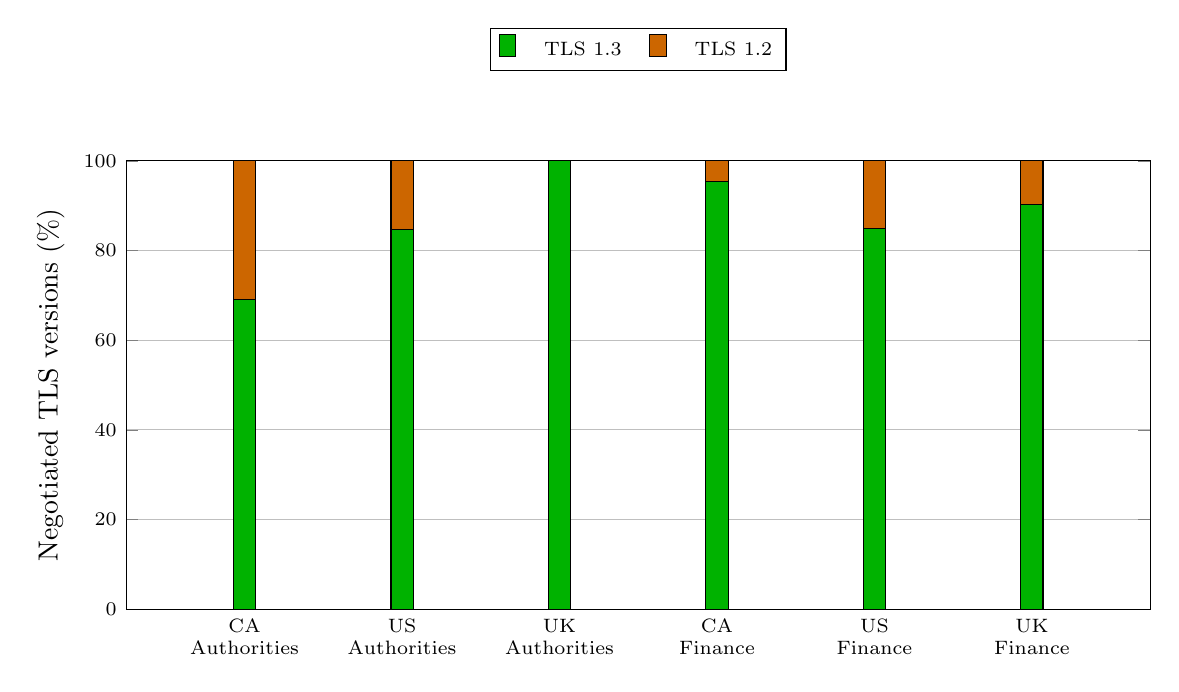
\begin{tikzpicture}
      \begin{axis}[
        ybar stacked,
        bar width=8pt,
        x=2cm,
        enlarge x limits=0.15,
        ymin=0, ymax=100,
        ylabel={Negotiated TLS versions (\%)},
        symbolic x coords={CA-Auth,US-Auth,UK-Auth,CA-Fin,US-Fin,UK-Fin},
        xtick=data,
        xticklabels={
          CA\\Authorities,
          US\\Authorities,
          UK\\Authorities,
          CA\\Finance,
          US\\Finance,
          UK\\Finance
        },
        xticklabel style={
          align=center,
          font=\scriptsize,
          text width=1.6cm
        },
        tick label style={font=\scriptsize},
        ymajorgrids=true,
        legend style={
          at={(0.5,1.20)},
          anchor=south,
          legend columns=3,
          column sep=8pt,
          font=\scriptsize,
        },
      ]

        \addplot[fill=green!70!black] coordinates {
          (CA-Auth, 69.1)
          (US-Auth, 84.6)
          (UK-Auth,100.0)
          (CA-Fin, 95.4)
          (US-Fin, 84.9)
          (UK-Fin, 90.2)
        };

        \addplot[fill=orange!80!black] coordinates {
          (CA-Auth, 30.9)
          (US-Auth, 15.4)
          (UK-Auth,  0.0)
          (CA-Fin,  4.6)
          (US-Fin, 15.1)
          (UK-Fin,  9.8)
        };

        \legend{TLS 1.3, TLS 1.2}
      \end{axis}
    \end{tikzpicture}}

    \caption{Stacked bar chart of negotiated TLS versions for authority and finance websites by country.}
    \label{fig:tls_stacked_auth_fin}
  \end{adjustbox}
\end{figure}


\subsubsection{Vulnerability Disclosure}

Table~\ref{tab:securitytxt_summary} reports security.txt adoption rates by dataset, including the presence of 
key fields such as Contact and Expires, and whether Expires values were valid.

\begin{table}[t]
  \caption{Security.txt adoption and field completeness by dataset.}
  \label{tab:securitytxt_summary}
  \centering
  \scriptsize
  \setlength{\tabcolsep}{2.2pt} 
  \renewcommand{\arraystretch}{1.15}

  \begin{adjustbox}{max width=\columnwidth}
  % \resizebox{\columnwidth}{!}{%
  \csvreader[
    tabular=lr rr ccc,
    table head=\toprule
      Dataset &
      $n$ orig. &
      \multicolumn{2}{c}{security.txt present} &
      Contact (\%) &
      Expires (\%) &
      Valid exp. (\%) \\
      \cmidrule(lr){3-4}
      & & Count & Share (\%) & & & \\\midrule,
    late after line=\\,
    late after last line=\\\bottomrule
  ]{../results/comparison/securitytxt/securitytxt_summary.csv}{%
    dataset_label=\Dataset,
    n_origins=\Norigins,
    n_with_securitytxt=\Nwith,
    pct_sites_with_securitytxt=\Psites,
    pct_with_contact_among_present=\Pcontact,
    pct_with_expires_among_present=\Pexpires,
    pct_valid_expires_among_expires=\Pvalid
  }{%
    \Dataset &
    \Norigins &
    \Nwith &
    \Psites &
    \Pcontact &
    \Pexpires &
    \Pvalid
  }%
  \end{adjustbox}
\end{table}

Among Canadian authority origins, only 1.1\% (4 of 375) 
published a security.txt file. All four files included Contact information and Expires fields, 
though only 25\% had unexpired dates. US authorities showed higher adoption at 3.5\% (13 of 373), 
with 92.3\% of those including Expires fields and 83.3\% maintaining valid expiration dates. 


\subsubsection{Security Headers \& Cookies}

Table~\ref{tab:security_headers_presence} summarizes adoption of selected security response
 headers at final resolved endpoints, including legacy hardening headers and modern user agent enforced policy controls.

\begin{table}[t]
  \caption{Security header adoption by dataset (percent of final URIs).}
  \label{tab:security_headers_presence}
  \centering
  \scriptsize
  \setlength{\tabcolsep}{2.2pt}
  \renewcommand{\arraystretch}{1.15}

  \begin{adjustbox}{max width=\columnwidth}
  % \resizebox{\columnwidth}{!}{%
  \csvreader[
    tabular=lccccc,
    table head=\toprule
      Dataset &
      \shortstack{Referrer\\Policy} &
      \shortstack{X-Content-Type\\Options} &
      \shortstack{X-Frame\\Options} &
      \shortstack{CSP\\frame-ancestors} &
      \shortstack{Permissions\\Policy} \\\midrule,
    late after line=\\,
    late after last line=\\\bottomrule
  ]{../results/comparison/headers/security_headers_presence.csv}{%
    dataset_label=\Dataset,
    pct_referrer_policy_present=\Pref,
    pct_x_content_type_options_present=\Pxcto,
    pct_x_frame_options_present=\Pxfo,
    pct_csp_frame_ancestors_present=\Pcsp,
    pct_permissions_policy_present=\Pperm
  }{%
    \Dataset & \Pref & \Pxcto & \Pxfo & \Pcsp & \Pperm
  }%
  \end{adjustbox}
  \end{table}

Table\ref{tab:cookie_security_flags} displays the cookie security attributes
 found among endpoints that set cookies as well as the fraction meeting the recommended/sufficient cookie profile. 
 These attributes including Secure, HttpOnly, and SameSite.

\begin{table}[t]
    \caption{Cookie security flag adoption by country and sector.}
    \label{tab:cookie_security_flags}
    \centering
    \scriptsize
    \setlength{\tabcolsep}{3pt}
    \renewcommand{\arraystretch}{1.15}
    
    \begin{adjustbox}{max width=\columnwidth}
    % \resizebox{\columnwidth}{!}{%
    \csvreader[
      tabular=lllrrr,
      table head=\toprule
        Dataset &
        Sites w/ cookies (\%) &
        Secure flag (\%) &
        HttpOnly flag (\%) &
        SameSite$\ge$Lax (\%) &
        Rec./Suff. (\%) \\\midrule,
      late after line=\\,
      late after last line=\\\bottomrule
    ]{../results/comparison/headers/cookie_security_flags_summary.csv}{%
      dataset_label=\Dataset,
      pct_sites_with_cookies=\Pcookies,
      pct_secure_among_cookie_sites=\Psecure,
      pct_httponly_among_cookie_sites=\Phttp,
      pct_samesite_ge_lax_among_cookie_sites=\Psame,
      pct_rec_suff_among_cookie_sites=\Prec
    }{%
      \Dataset & \Pcookies & \Psecure & \Phttp & \Psame & \Prec
    }%
    \end{adjustbox}
  \end{table}

28.2\% of Canadian authority sites set cookies, of which 63.5\% set Secure, 48.7\% set HttpOnly, and 15.7\% set SameSite $\geq$ Lax.
Only 3.5\% of Canadian authority cookie-setting sites met the recommended/sufficient cookie configuration criteria. 


\subsubsection{Information Leakage}

Table~\ref{tab:revealing_headers_summary} illustrates the distribution of 
technology-revealing response headers per origin, including the share exposing
 at least one such header.

    \begin{table}[t]
      \caption{Distribution of technology-revealing headers by dataset.}
      \label{tab:revealing_headers_summary}
      \centering
      \scriptsize
      \setlength{\tabcolsep}{3pt}
      \renewcommand{\arraystretch}{1.15}
    
      \begin{adjustbox}{max width=\columnwidth}
      % \resizebox{\columnwidth}{!}{%
      \csvreader[
        tabular=lrrrrrc,
        table head=\toprule
          Dataset &
          $n$ sites &
          \multicolumn{4}{c}{$n$ revealing headers (\%)} &
          Any (\%) \\
          \cmidrule(lr){3-6}
          & & 0 & 1 & 2 & 3+ & \\\midrule,
        late after line=\\,
        late after last line=\\\bottomrule
      ]{../results/comparison/headers/revealing_headers_summary.csv}{%
        dataset_label=\Dataset,
        n_sites=\Nsites,
        pct_revealing_0=\Pzero,
        pct_revealing_1=\Pone,
        pct_revealing_2=\Ptwo,
        pct_revealing_3_plus=\Pthree,
        pct_with_any_revealing=\Pany
      }{%
        \Dataset &
        \Nsites &
        \Pzero &
        \Pone &
        \Ptwo &
        \Pthree &
        \Pany
      }%
      \end{adjustbox}
    \end{table}
    
Lastly, the table below illustrates the leaks found in each origin's error page responses.
94.4\% of Canadian authority origins exposed at least one technology-revealing header, with 10.8\% exposing three or more.
Notably, all sectors and jurisdictions showed a majority of origins leaking revealing headers. Table~\ref{tab:error_leaks_summary} reports the prevalence
 of leaked technology in error responses and pages.

    % Error Leaks Summary Table
    \begin{table}[t]
      \caption{Information leakage in HTTP error responses by dataset.}
      \label{tab:error_leaks_summary}
      \centering
      \scriptsize
      \setlength{\tabcolsep}{4pt}
      \renewcommand{\arraystretch}{1.15}
      
      \begin{adjustbox}{max width=\columnwidth}
      % \resizebox{\columnwidth}{!}{%
      \csvreader[
        tabular=lrrr,
        table head=\toprule
          Dataset &
          $n$ origins &
          Any tech leak (\%) &
          Version leak (\%) \\\midrule,
        late after line=\\,
        late after last line=\\\bottomrule
      ]{../results/comparison/error_leaks/error_leaks_summary.csv}{%
        dataset_label=\Dataset,
        n_scanned_origins=\Norigins,
        pct_any_tech_leak=\Ptech,
        pct_version_leak=\Pversion
      }{%
        \Dataset & \Norigins & \Ptech & \Pversion
      }%
      \end{adjustbox}
    \end{table}
        

In Canadian authorities, 47.2\% of origins exhibited technology leakage in error responses, and 10.7\% disclosed explicit version information.
Comparable leakage rates were observed across most datasets, including 44.5\% and 50.0\% in US and UK authorities respectively.


\section{Discussion}\label{sec:discussion}


This study measured the adoption of transport and browser-enforced web security controls across Canadian public-sector and
critical-sector sites, with cross-jurisdiction comparisons to the United States and United Kingdom.
Overall, baseline transport security is widely deployed across most datasets, but
adoption is uneven in Canadian authorities and stronger controls are not consistently enforced.
Across sectors, modern browser-side hardening remains sparse relative to transport-level adoption. 
Furthermore, technology disclosure through response metadata and error handling remains common,
indicating that low-effort fingerprinting opportunities still persist even where HTTPS is present.

    
First, the results show that transport protections are common but not ubiquitous. 
Most measured origins are HTTPS-reachable and the majority of HTTP-accessible services upgrade users to HTTPS (Table~\ref{tab:https_connectivity}), 
indicating that HTTPS is now the default for much of the Canadian web. Within Canada, non-authority datasets typically
show stronger transport reachability behavior than authorities (Table~\ref{tab:https_connectivity}).  
Moreover, in all datasets most services upgrade users via redirection (Table~\ref{tab:https_connectivity}),
yet a substantial portion of Canadian authority sites still serve HTTP without upgrading (6.43\%). Likewise, Canadian
authorities remain the lowest-performing Canadian sector on TLS~1.3 compatability and default negotiation (Fig.~\ref{fig:tls_stacked_auth_fin}). 
Accross jurisdictions, TLS configurations remained quite strong, although a considerable portion still advertises legacy TLS protocol support (Table~\ref{tab:tls_summary}). 
Most sites in all jurisdictions naturally negotiated the widely recommended TLS~1.3, with 0\% of sites negotiating legacy TLS.

Browser-enforced controls show the largest adoption gaps. At the application layer, Canadian authority endpoints more frequently implement legacy hardening
 headers such as \texttt{X-Frame-Options} and \texttt{X-Content-Type-Options} than modern policy controls, with notably weaker adoption
 of CSP \texttt{frame-ancestors} and \texttt{Permissions-Policy} (Table~\ref{tab:security_headers_presence}). HSTS adoption among Canadian
authority sites is on the lower-end, with over 40\% of sites not supporting HSTS, and of those only 27.43\% appear on the preload list (Table~\ref{tab:https_hsts_quality}).
Accross all datsets, the fraction of cookies that meet recommended or sufficient attribute profiles was found to be extremely small
 (only 3.5\% for CA authorities) (Table~\ref{tab:cookie_security_flags}).

Similarlities are present in both information leakage and vulnerability disclosure. A substantial fraction of all datasets contain revealing headers and
leak technology information in error responses. Additionally, a non-trivial fraction leak version information, including nearly 50\% of the Canadian authority sites evaluated (Table~\ref{tab:revealing_headers_summary} and Table~\ref{tab:error_leaks_summary}). 
Notably, near-zero origins hosted a \texttt{security.txt} file in all datasets, despite the prevalence of information leakage. Regarding Canadian authorities, 
only 4 of 375 origins were found to host a \texttt{security.txt} file, of which 75\% contained an expired Expires field (Table~\ref{tab:securitytxt_summary}). 
This combination is especially consequential because it lowers the cost of reconnaissance while simultaneously reducing the likelihood that external researchers 
can report issues through a standardized channel.


\subsection{Conclusion}

Importantly, these are not exotic mitigations. Many are low-effort, configuration-driven controls 
that can be deployed at the edge (CDN/WAF/reverse proxy) without application rewrites. The results suggest that the gaps found in 
Canadian web security is not a lack of
technical capability, but inconsistent adherence to existing guidance. The CCCS publishes comprehensive, 
and pragmatic recommendations for securing both the transport and application layer of HTTP. However, the
contrast with US federal practice is apparent. Our cross-country results 
reflect the difference in governance models found in the UK and US. The results illustrate a higher and more uniform 
adoption of the same controls in the US and UK, despite them being recommended in Canada. Web configuration and development 
is complex and web development remains one of the most rapidly changing areas of IT. Converting recommendations 
into consistently applied practice would reduce exposure to common attacks and better
honour the trust that Canadians place in online public services.


\subsection{Limitations}

This measurement study has several limitations. First, results reflect the scanner’s network vantage point and
strict ethical rate limits. Some ``unreachable'' outcomes may reflect bot mitigation or WAF policies rather than
service unavailability. However, from an external user perspective, aggressive filtering can still function as a
practical availability barrier, and therefore remains relevant to posture. Second, our header and cookie analysis
was performed on landing-page responses. Some sites may apply stricter controls on authenticated or transactional
paths. Third, \texttt{security.txt} discovery did not follow cross-origin redirects, which may undercount sites
that host disclosure policy on centralized origins. Finally, this study evaluates security control adoption rather
than exploitability: absence of a control indicates increased risk exposure, but not necessarily the presence of a
specific vulnerability.

\subsection{Future Work}

Future work should extend this benchmarking methodology in three directions. First, longitudinal scans would
quantify change over time and assess whether policy interventions measurably improve posture. 
Second, expanding endpoint coverage beyond landing pages (e.g., authentication and high-value workflows) would better capture how
controls vary across application surfaces. Third, deeper dependency analysis could quantify third-party resource
exposure and content supply-chain risk, complementing prior findings that government sites often rely on external
infrastructure \cite{hsiao2019cyberautonomy}. Together, these extensions would enable continuous measurement of
Canada’s public-sector web security maturity, supporting both operational remediation and evidence-based policy.

\section*{Acknowledgment}

% The preferred spelling of the word ``acknowledgment'' in America is without 
% an ``e'' after the ``g''. Avoid the stilted expression ``one of us (R. B. 
% G.) thanks $\ldots$''. Instead, try ``R. B. G. thanks$\ldots$''. Put sponsor 
% acknowledgments in the unnumbered footnote on the first page.

% \section*{References}

\bibliographystyle{IEEEtran}
\bibliography{main}

% Please number citations consecutively within brackets \cite{b1}. The 
% sentence punctuation follows the bracket \cite{b2}. Refer simply to the reference 
% number, as in \cite{b3}---do not use ``Ref. \cite{b3}'' or ``reference \cite{b3}'' except at 
% the beginning of a sentence: ``Reference \cite{b3} was the first $\ldots$''

% Number footnotes separately in superscripts. Place the actual footnote at 
% the bottom of the column in which it was cited. Do not put footnotes in the 
% abstract or reference list. Use letters for table footnotes.

% Unless there are six authors or more give all authors' names; do not use 
% ``et al.''. Papers that have not been published, even if they have been 
% submitted for publication, should be cited as ``unpublished'' \cite{b4}. Papers 
% that have been accepted for publication should be cited as ``in press'' \cite{b5}. 
% Capitalize only the first word in a paper title, except for proper nouns and 
% element symbols.

% For papers published in translation journals, please give the English 
% citation first, followed by the original foreign-language citation \cite{b6}.

% \begin{thebibliography}{00}
% \bibitem{b1} G. Eason, B. Noble, and I. N. Sneddon, ``On certain integrals of Lipschitz-Hankel type involving products of Bessel functions,'' Phil. Trans. Roy. Soc. London, vol. A247, pp. 529--551, April 1955.
% \bibitem{b2} J. Clerk Maxwell, A Treatise on Electricity and Magnetism, 3rd ed., vol. 2. Oxford: Clarendon, 1892, pp.68--73.
% \bibitem{b3} I. S. Jacobs and C. P. Bean, ``Fine particles, thin films and exchange anisotropy,'' in Magnetism, vol. III, G. T. Rado and H. Suhl, Eds. New York: Academic, 1963, pp. 271--350.
% \bibitem{b4} K. Elissa, ``Title of paper if known,'' unpublished.
% \bibitem{b5} R. Nicole, ``Title of paper with only first word capitalized,'' J. Name Stand. Abbrev., in press.
% \bibitem{b6} Y. Yorozu, M. Hirano, K. Oka, and Y. Tagawa, ``Electron spectroscopy studies on magneto-optical media and plastic substrate interface,'' IEEE Transl. J. Magn. Japan, vol. 2, pp. 740--741, August 1987 [Digests 9th Annual Conf. Magnetics Japan, p. 301, 1982].
% \bibitem{b7} M. Young, The Technical Writer's Handbook. Mill Valley, CA: University Science, 1989.
% \end{thebibliography}
% \vspace{12pt}
% \color{red}
% IEEE conference templates contain guidance text for composing and formatting conference papers. Please ensure that all template text is removed from your conference paper prior to submission to the conference. Failure to remove the template text from your paper may result in your paper not being published.

\end{document}
